\documentclass{beamer}
\usepackage[utf8]{inputenc}
\usepackage[T2A]{fontenc}
\usepackage[english,russian]{babel}
\usepackage{graphicx} % Пакет для работы с изображениями
\usepackage{adjustbox} % Hyperlinks

\usetheme{Warsaw}

\setbeamertemplate{footline}[frame number]

\begin{document}

\begingroup
\setbeamertemplate{footline}{}

\begin{frame}
\begin{center}
\Large РАЗРАБОТКА БАЗЫ ДАННЫХ ДЛЯ АВТОМАТИЗАЦИИ РАБОЧЕГО МЕСТА РАЗМЕТЧИКОВ ПАРАЛЛЕЛЬНОГО КОРПУСА ТЕХНИЧЕСКИХ ТЕКСТОВ
\end{center}

\vfill

\begin{minipage}[t]{0.45\textwidth}
    \raggedright
    Выполнил:

    студент 3 курса

    группы ИУ7-64Б

    \makebox[0pt][l]{Рунов Константин Алексеевич}
\end{minipage}
\hfill
\begin{minipage}[t]{0.45\textwidth}
    \raggedleft
    Руководитель:

    \makebox[0pt][r]{Строганов Юрий Владимирович}
\end{minipage}

\vfill

\begin{center}
    Москва, \the\year\ г.
\end{center}
\end{frame}
\endgroup

\begin{frame}
    \frametitle{Цель и задачи}
    Цель: Разработать базу данных для автоматизации рабочего места разметчиков параллельного корпуса технических текстов.

    \vfill

    Задачи:
    \begin{itemize}
        \item Провести анализ предметной области корпусов текстов;
        \item Спроектировать и разработать базу данных, описать ее сущности, ограничения целостности, ролевую модель на уровне базы данных и используемые триггеры;
        \item Разработать приложение для доступа к базе данных;
        \item Исследовать зависимость времени ответа от количества запросов в секунду и сравнить эффективности реализаций приложения с использованием дополнительного кеширования и без него.
    \end{itemize}
\end{frame}

\begin{frame}
    \frametitle{Введение в предметную область и существующие проблемы}
    Рассказ про корпуса текстов, разметки, проблему терминов, про то что на данный момент в принципе не существует корпусов технических текстов...
\end{frame}

\begin{frame}
    \frametitle{Существующие аналоги}
    Примеры существующих корпусов и автоматических разметчиков со скриншотами, но в итоге сказать, что все равно нет корпусов технических текстов...
\end{frame}

\begin{frame}
    \frametitle{Диаграмма сущностей}
    \centering
	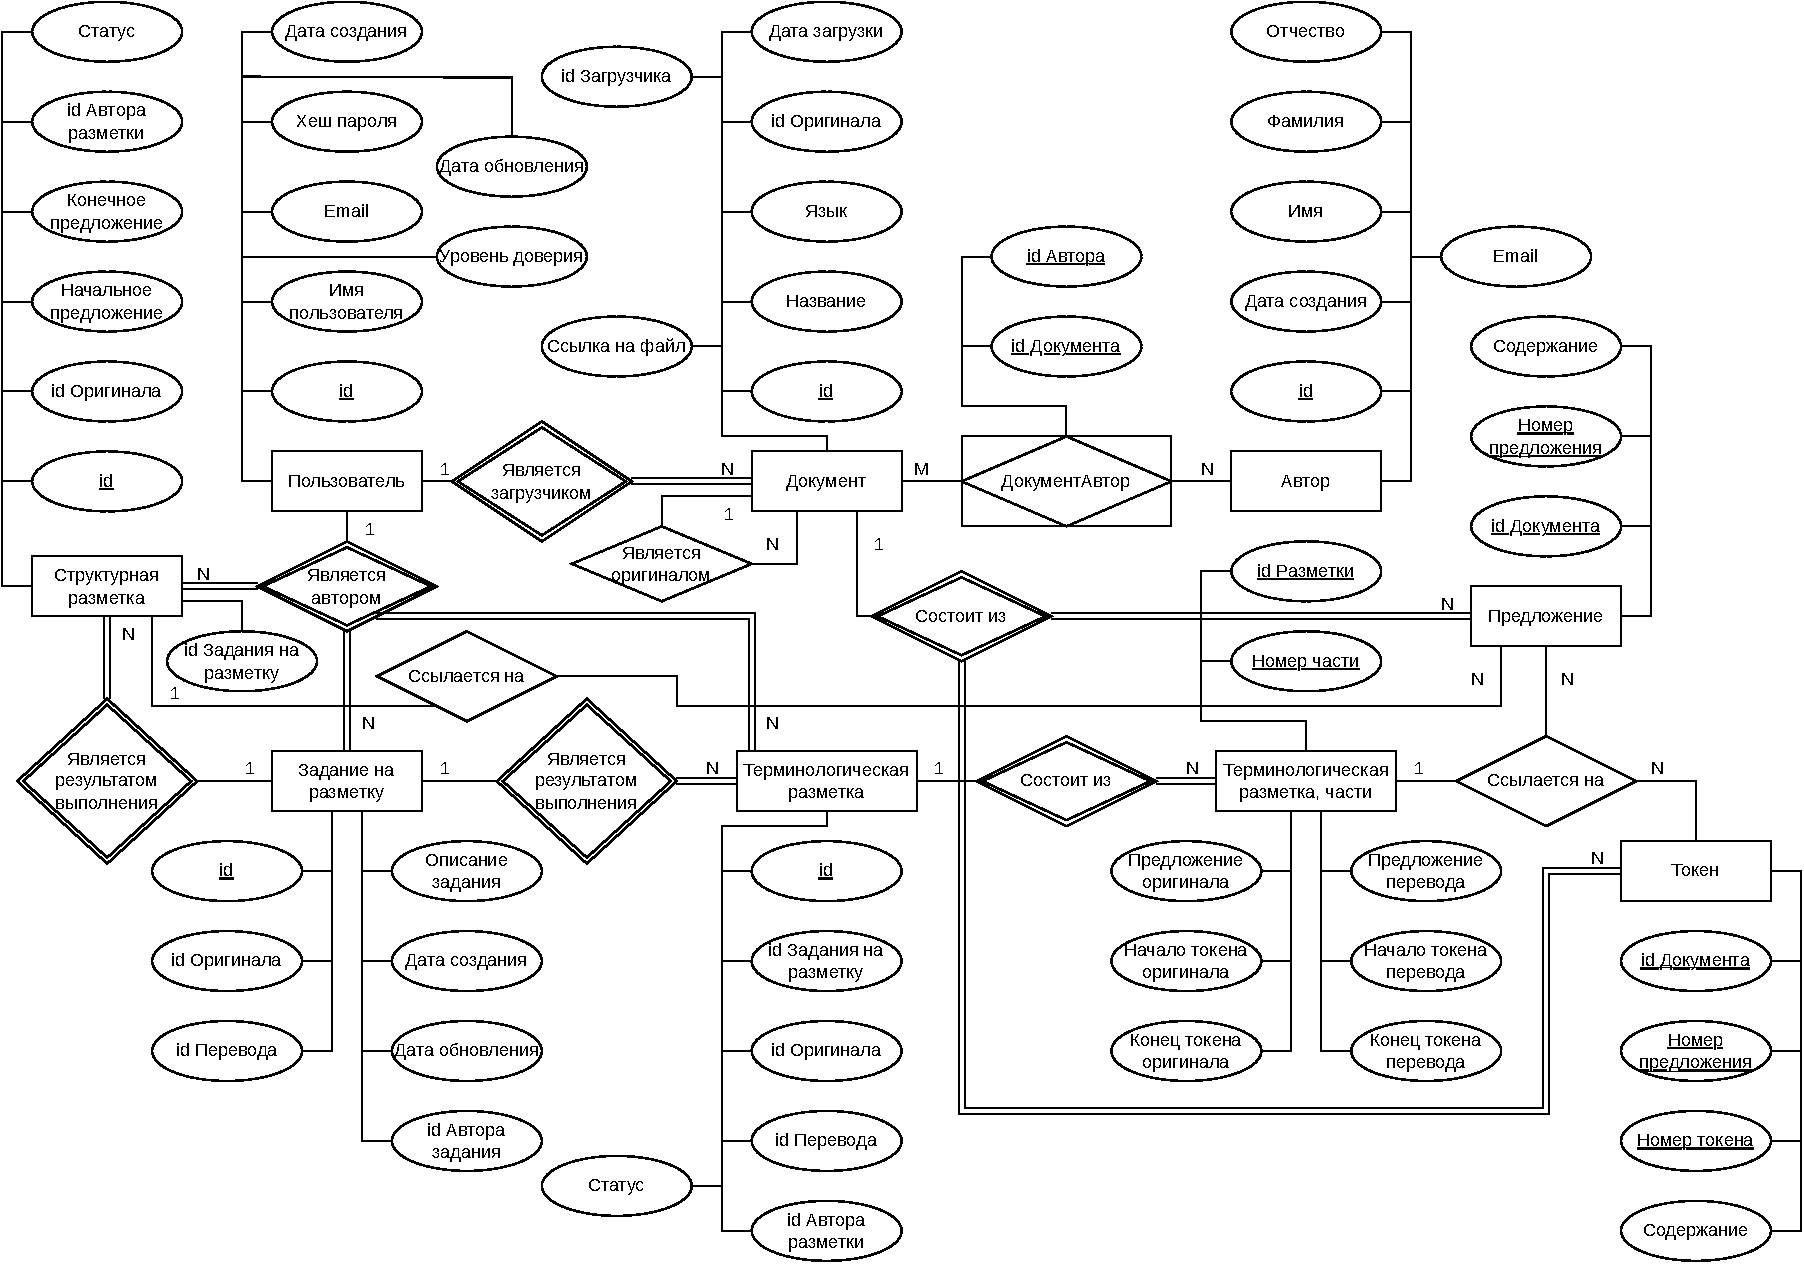
\includegraphics[width=\textwidth]{diag/chen-v9.pdf}
\end{frame}

\begin{frame}
    \frametitle{Диаграмма вариантов использования}
    \centering
	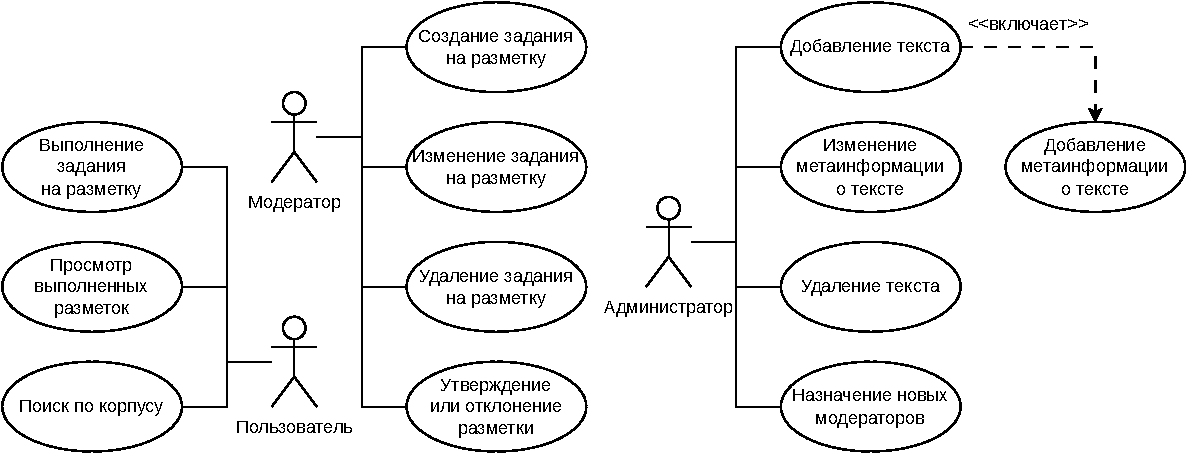
\includegraphics[width=\textwidth]{diag/use-case-v2.pdf}
\end{frame}

\begin{frame}
    \frametitle{Диаграмма проектируемой БД}
    \centering
	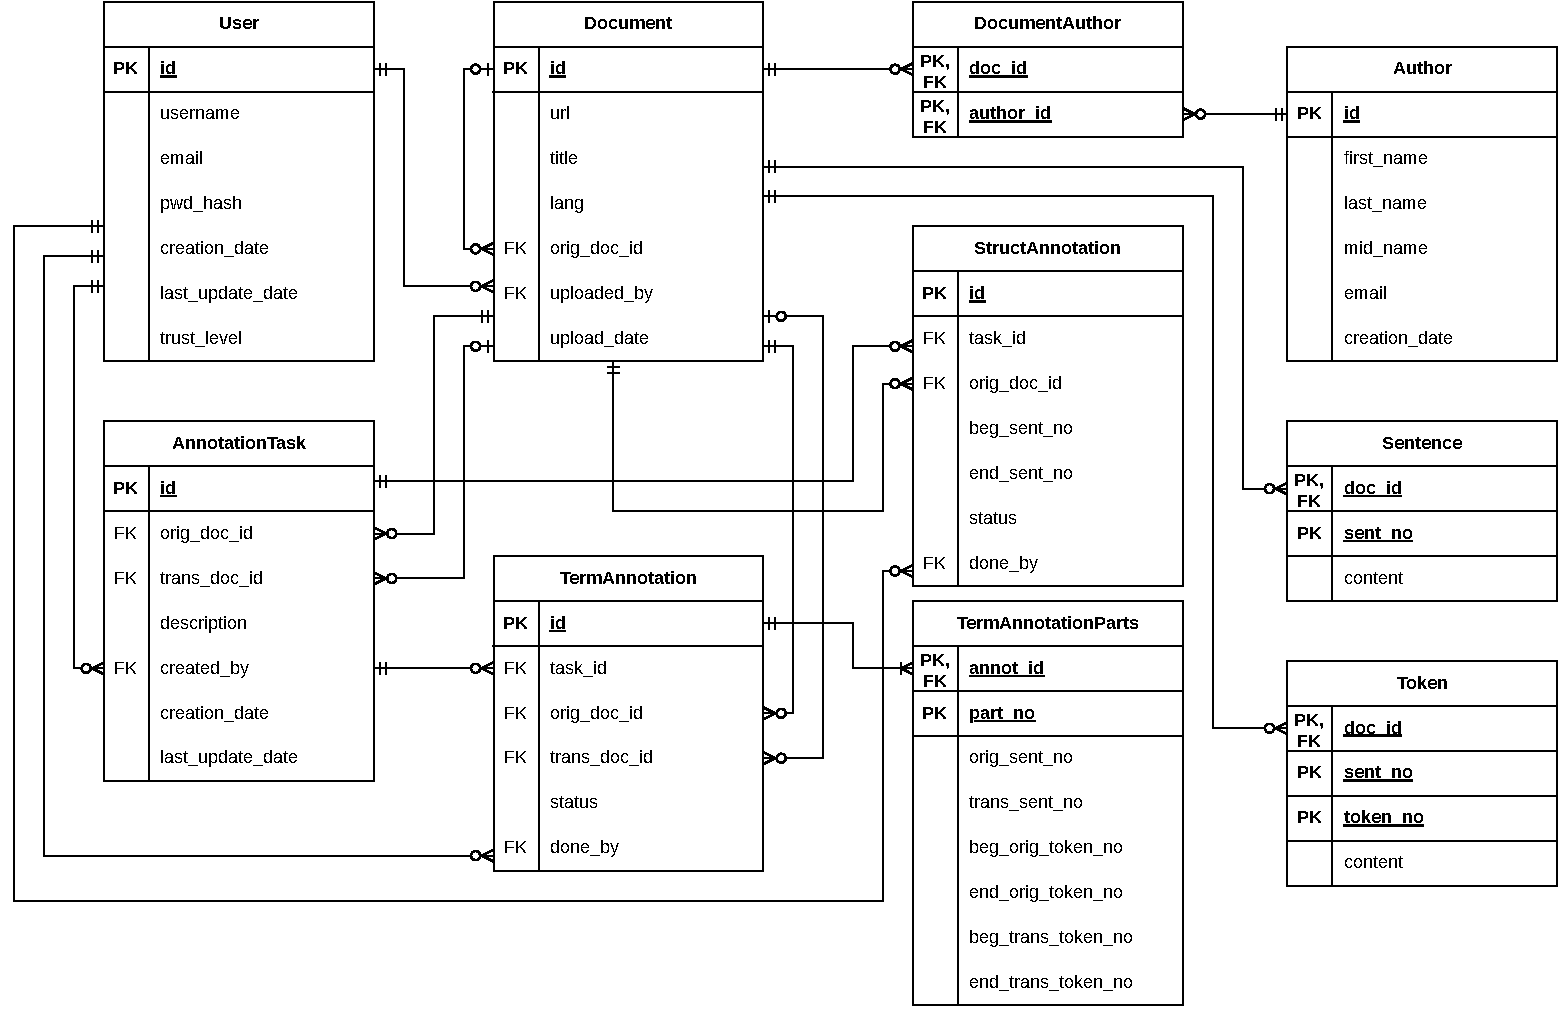
\includegraphics[width=\textwidth]{diag/erd-v3.pdf}
\end{frame}

\begin{frame}
    \frametitle{Схема проектируемого триггера}
    \centering
	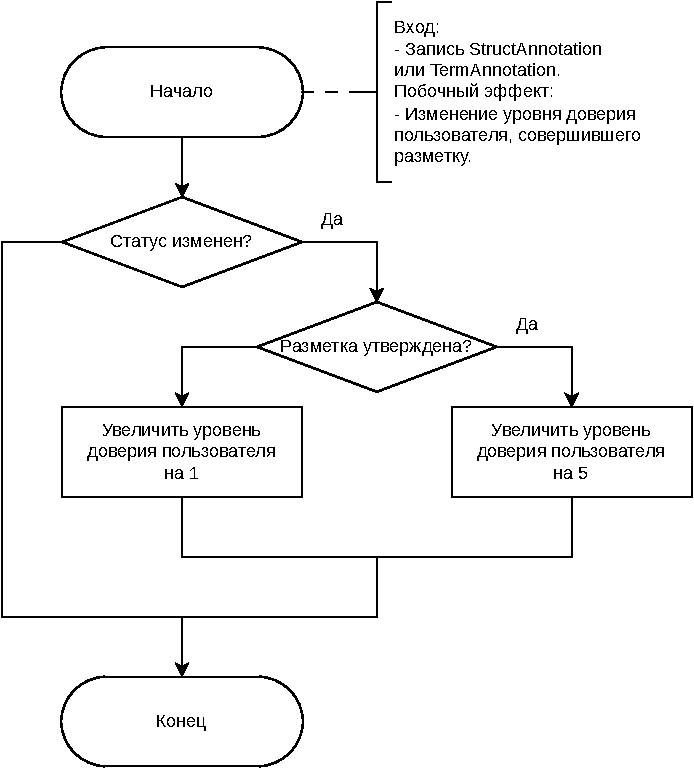
\includegraphics[width=0.6\textwidth]{diag/trig-v4.pdf}
\end{frame}

\begin{frame}
    \frametitle{Схема реализованного триггера}
    \centering
	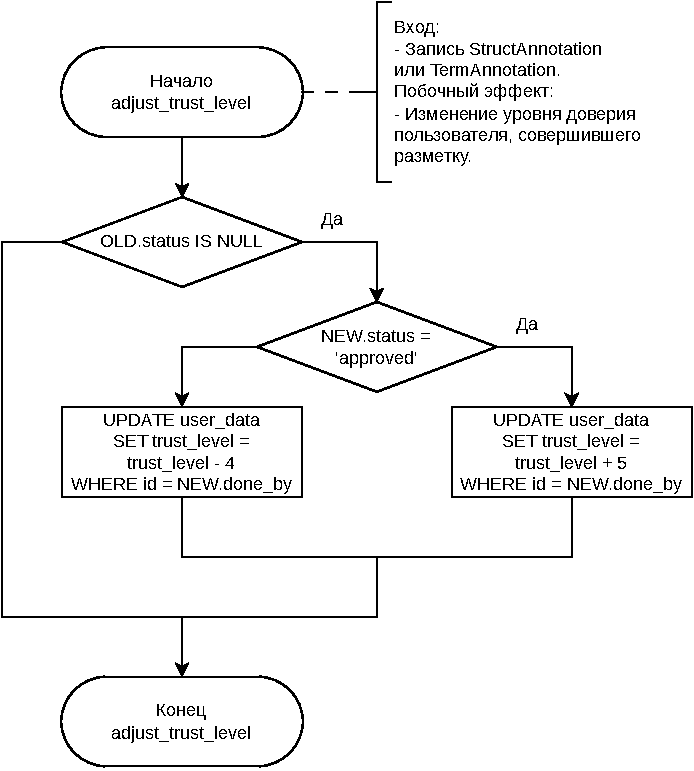
\includegraphics[width=0.6\textwidth]{diag/tech-trig-v4.pdf}
\end{frame}

\begin{frame}
    \frametitle{Результаты исследования}
    \centering
	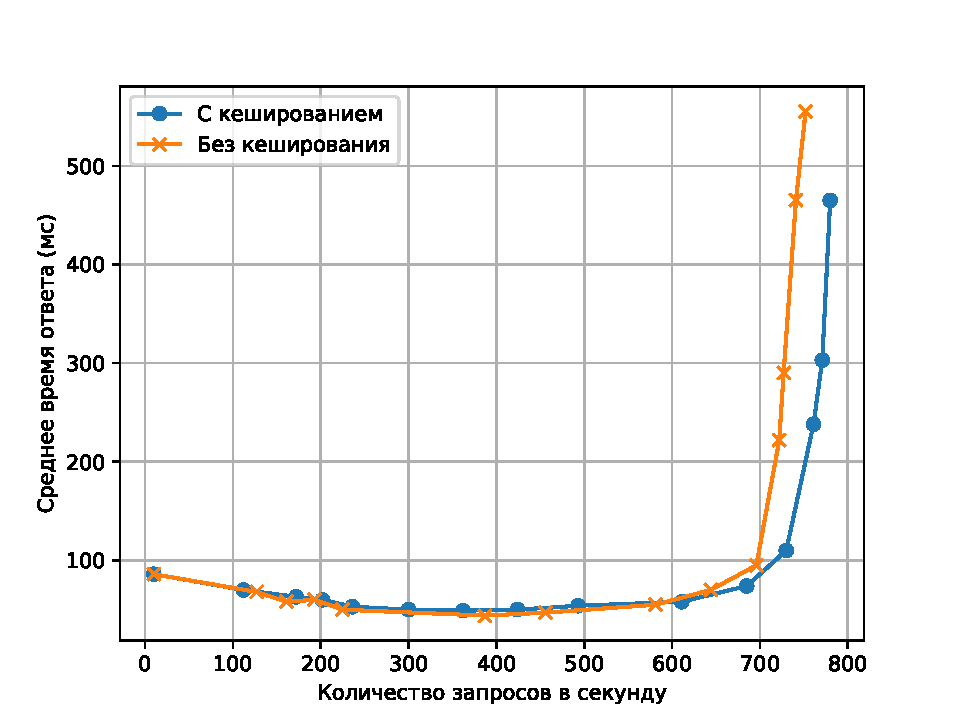
\includegraphics[width=0.9\textwidth]{img/avg-resp-time.pdf}
    Числа...
\end{frame}

\begin{frame}
    \frametitle{Результаты исследования}
    \centering
	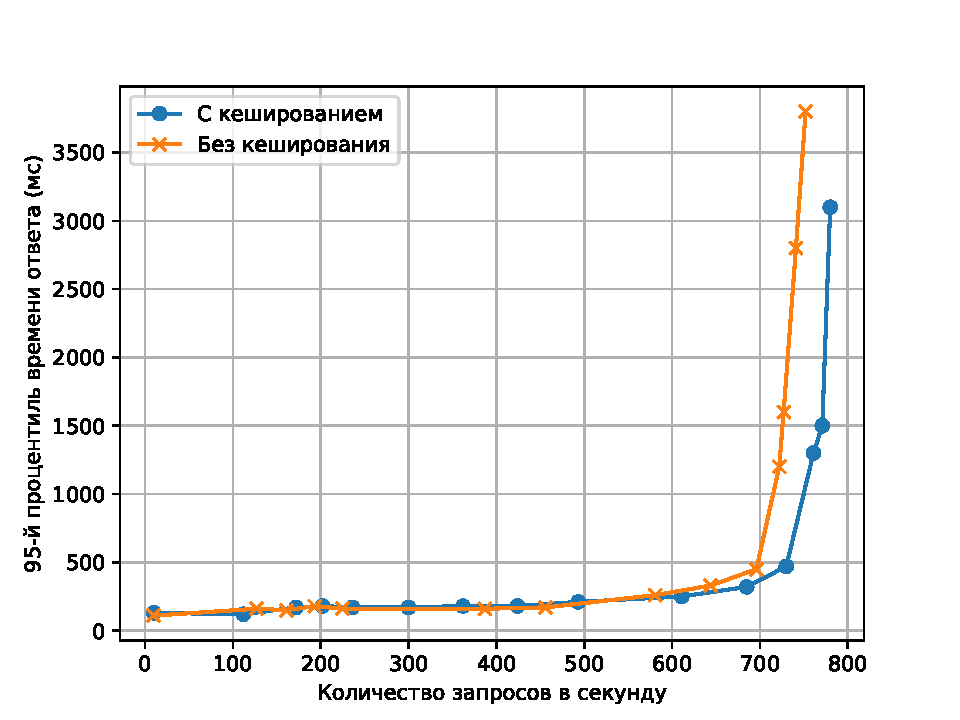
\includegraphics[width=0.9\textwidth]{img/95-resp-time.pdf}
    Числа...
\end{frame}

\begin{frame}
    \frametitle{Заключение}
\end{frame}

\begin{frame}
    \frametitle{Направления дальнейшего развития}
    Разработать нормальное приложение для спроектированной базы данных...
\end{frame}

\end{document}
